\section{Organizational Breakdown Structure}
\label{dsePPOBS}
The organizational breakdown can be found in figure \ref{organogram} on page \pageref{organogram}. The diagram has been divided into two logical parts: management and technical responsibilities.

The managerial responsibilities are as follows:
\begin{itemize}
	\item Chairman - responsible for keeping the project on track and accountable for all deliverables. He is furthermore entrusted with making sure all the meetings are organized and that all members are aware of their respective tasks.
	\item Secretary - keeps track of all discussions and decisions made at meetings. Furthermore he is responsible for logistics as well as communications with the tutor.
	\item Systems Engineer - responsible for systems engineering content.
	\item Archiver - responsible for organizing and overseeing IT resources to be used for data storage and report writing.
	\item Quality Assurance Officer - responsible for report content.
	\item External Relations Officer - responsible for external party relations.
	\item Sustainable Engineer - responsible for sustainable development guidance. 
\end{itemize}

%\newpage
\begin{figure}[H]
\begin{center}

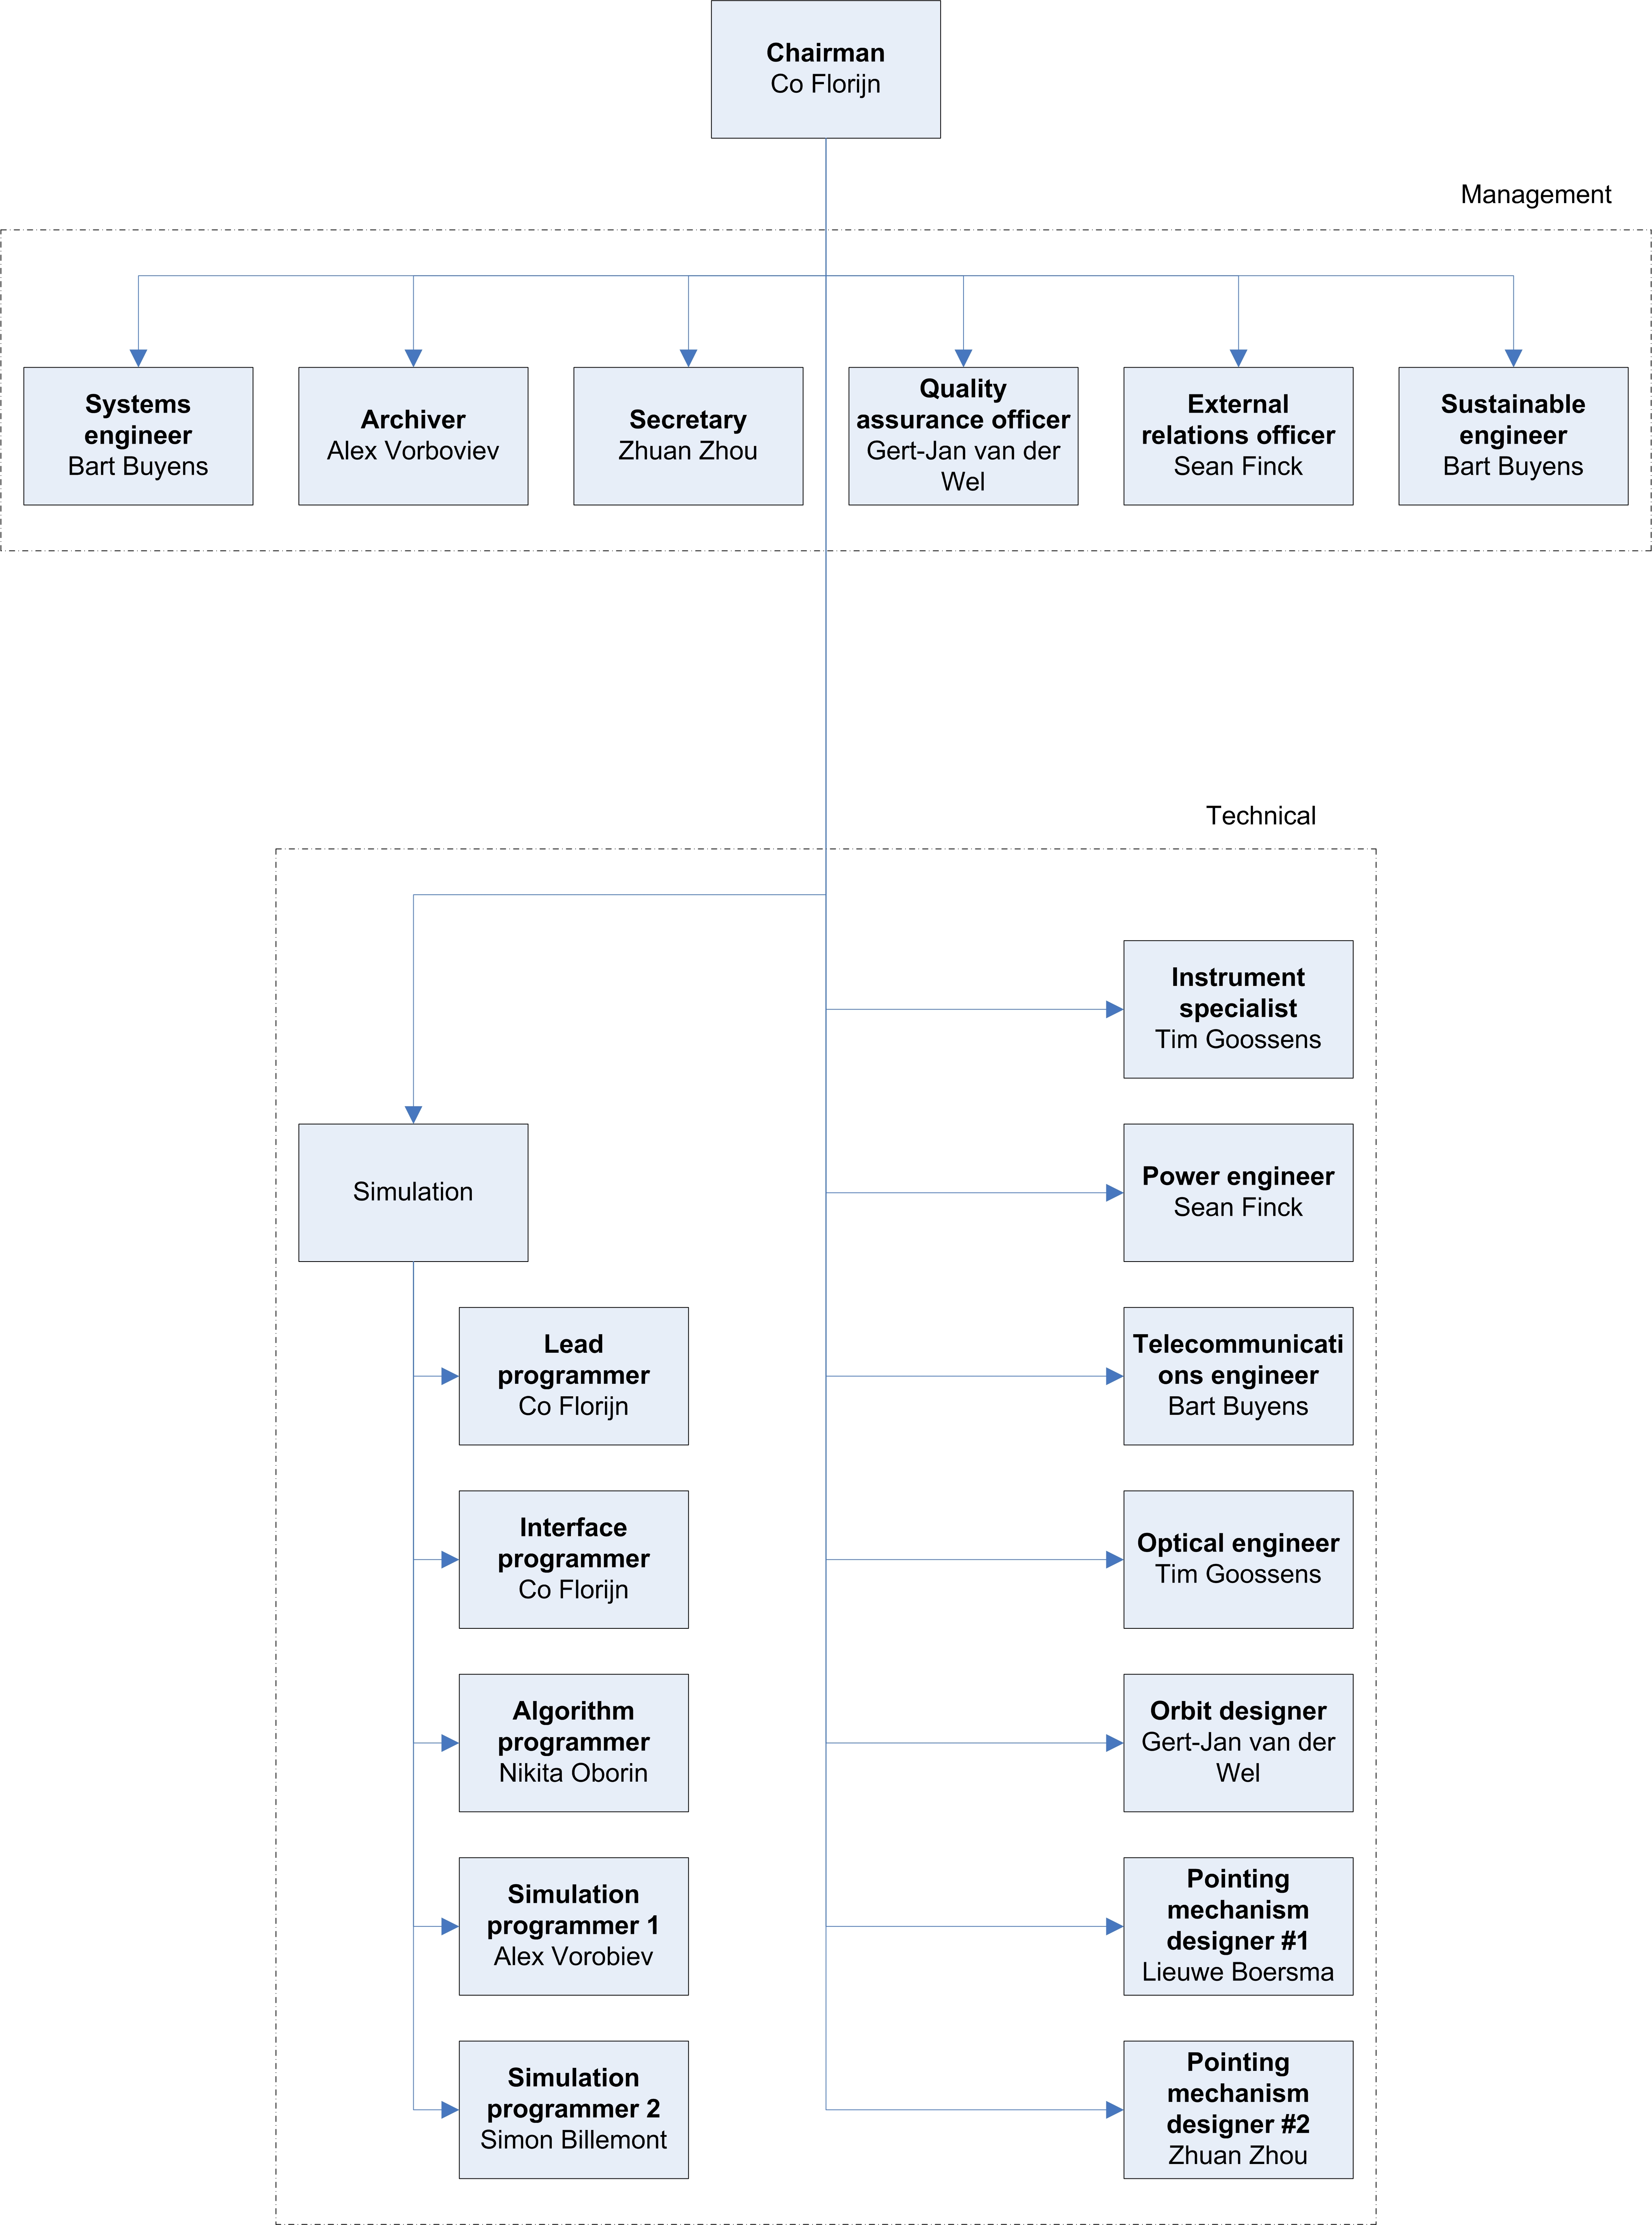
\includegraphics[scale=0.8]{chapters/img/Organogram.jpg}
\caption{Organogram}
\label{organogram}
\end{center}
\end{figure}